\documentclass[aspectratio=169, t, 8pt]{beamer}

%------configurando acentos-----------
\usepackage[utf8]{inputenc}
\usepackage[T1]{fontenc}
\usepackage[brazil]{babel}
\usepackage{montserrat}
\usefonttheme[onlymath]{serif}
\usepackage{booktabs} % Tabelas elegantes sem linhas verticais
\usepackage[most]{tcolorbox}
\usepackage{graphicx}

%-------Estilos Beamer---------------
\usetheme{metropolis}
%\usecolortheme{crane}
%\usefonttheme{serif}
\linespread{1.2}

% Personalização de Cores (Exemplo: Minimal Teal)
% Cores Base
\definecolor{BgCanvas}{HTML}{F9F9FB}      % Off-white muito suave
\definecolor{MainText}{HTML}{2B2D42}      % Grafite escuro para alta legibilidade
\definecolor{PrimaryAccent}{HTML}{4A6FA5} % Azul poeira (Dusty Blue)

% Tons Pastéis para Destaques e Cards
\definecolor{PastelGreenBg}{HTML}{E8F0EC}  % Sálvia Claro (Sucesso / Destaque Positivo)
\definecolor{PastelGreenFg}{HTML}{2D5A44}

\definecolor{PastelCoralBg}{HTML}{FDEAE6}  % Coral Soft (Atenção / Problema / Alerta)
\definecolor{PastelCoralFg}{HTML}{7A3025}

\definecolor{PastelPurpleBg}{HTML}{F0EBF4} % Lavanda (Conceitos / Citações)
\definecolor{PastelPurpleFg}{HTML}{4A3E56}

\definecolor{PastelYellowBg}{HTML}{FFF4E6} % Areia / Manteiga (Notas / Dados Secundários)
\definecolor{PastelYellowFg}{HTML}{7A522A}

% --- CONFIGURAÇÕES DE TEMA BEAMER ---
%\usetheme{metropolis}

\setbeamertemplate{itemize item}{\textcolor{MainText}{$\bullet$}}
\setbeamertemplate{itemize subitem}{\textcolor{MainText}{\scriptsize$\circ$}}
\setbeamertemplate{itemize 3rditem}{\textcolor{MainText}{\tiny$\blacksquare$}}

\setbeamercolor{background canvas}{bg=BgCanvas}
\setbeamercolor{normal text}{fg=MainText}
\setbeamercolor{frametitle}{bg=PastelGreenFg, fg=BgCanvas}
\setbeamercolor{title}{fg=MainText}
\setbeamercolor{subtitle}{fg=PrimaryAccent}
\setbeamercolor{structure}{fg=PrimaryAccent}

% Remove a linha amarela padrão do Metropolis sob o título
\setbeamertemplate{title separator}{}
\setbeamertemplate{progress bar in section page}{}

% ==============================================================================
% PALETA DE CORES "GEOMETRIA AQUECIDA" (Inspirada na imagem)
% ==============================================================================
\definecolor{BgCream}{HTML}{FFFDFB}       % Fundo creme suave
\definecolor{TextDark}{HTML}{2C1A14}      % Texto em castanho escuro elegante
\definecolor{PrimaryOrange}{HTML}{E0531C}  % Laranja vibrante (Títulos e destaques)
\definecolor{Terracotta}{HTML}{B8380D}     % Terracota queimado (Alertas)
\definecolor{SoftOrange}{HTML}{FFE6D5}     % Laranja bem suave (Fundo de blocos)

% ==============================================================================
% CONFIGURAÇÃO DO TEMA METROPOLIS
% ==============================================================================
% Cores do texto e fundo geral
\setbeamercolor{normal text}{fg=TextDark, bg=BgCream}
\setbeamercolor{alerted text}{fg=Terracotta}
\setbeamercolor{example text}{fg=PrimaryOrange}

% Barra de título dos slides (Frametitle)
\setbeamercolor{frametitle}{fg=BgCream, bg=PrimaryOrange}

% Título principal da apresentação (Slide de Capa)
\setbeamercolor{titlelike}{fg=PrimaryOrange}
\setbeamercolor{subtitle}{fg=Terracotta}

% Barra de progresso (Linha do Metropolis)
\setbeamercolor{progress bar}{fg=PrimaryOrange, bg=PrimaryOrange!20}

% Customização de Blocos (block, alertblock, exampleblock)
\setbeamercolor{block title}{fg=BgCream, bg=PrimaryOrange}
\setbeamercolor{block body}{fg=TextDark, bg=SoftOrange}

\setbeamercolor{block title alerted}{fg=BgCream, bg=Terracotta}
\setbeamercolor{block body alerted}{fg=TextDark, bg=Terracotta!15}


% --- ESTILOS DE CARDS PASTEL COM TCOLORBOX ---
\newtcolorbox{cardPrincipal}[1][]{
  colback=SoftOrange,
  colframe=Terracotta,
  coltext=TextDark,
  arc=6pt,
  boxrule=0pt,
  left=12pt, right=12pt, top=10pt, bottom=10pt,
  fonttitle=\bfseries\small,
  #1
}

\newtcolorbox{cardcoral}[1][]{
  colback=PastelCoralBg,
  colframe=PastelCoralFg,
  coltext=PastelCoralFg,
  arc=6pt,
  boxrule=0pt,
  left=12pt, right=12pt, top=10pt, bottom=10pt,
  fonttitle=\bfseries\small,
  #1
}

\newtcolorbox{cardpurple}[1][]{
  colback=PastelPurpleBg,
  colframe=PastelPurpleFg,
  coltext=PastelPurpleFg,
  arc=6pt,
  boxrule=0pt,
  left=12pt, right=12pt, top=10pt, bottom=10pt,
  fonttitle=\bfseries\small,
  #1
}

\newtcolorbox{cardyellow}[1][]{
  colback=PastelYellowBg,
  colframe=PastelYellowFg,
  coltext=PastelYellowFg,
  arc=6pt,
  boxrule=0pt,
  left=12pt, right=12pt, top=10pt, bottom=10pt,
  fonttitle=\bfseries\small,
  #1
}

\graphicspath{{../../src/img/semana04/}}

%--------Dados do Documento
\title{Geometria: Perímetro e Área de Figuras Planas}
\subtitle{}
\author{prof. Eduardo}
\institute{Pré-Universitário Oficina do Saber / UFF}

\date{\today}


%-------- Pacotes Matemática -------------
\usepackage{amsmath}
\usepackage{amsthm}
\usepackage{amsfonts}
\usepackage{amssymb}
\usepackage{xfrac}
\usepackage{thmtools}

\begin{document}

    \begin{frame} %capa
        \vspace*{\fill}
            
            \begin{columns}[c]
                \begin{column}{0.5\textwidth}
                    {\usebeamerfont{title}\usebeamercolor[fg]{title}\inserttitle}\vspace{0.2cm}
                    
                    {\usebeamerfont{subtitle}\usebeamercolor[fg]{subtitle}\insertsubtitle}\vspace{0.5cm}

                {\usebeamerfont{author}\insertauthor}\vspace{0.3cm}

                {\usebeamerfont{institute}\insertinstitute}\vspace{0.3cm}

                {\usebeamerfont{date}\insertdate}
            \end{column}
            
            
            \begin{column}{0.4\textwidth}
                \centering
                
\includegraphics[width=0.4\textwidth]{../logo_ofSaber.png}

                \vspace{.4cm}
                \vspace*{\fill}
        \begin{columns}[c]
            \begin{column}{.5\textwidth}
                \centering
\includegraphics[width=.5\textwidth]{../Proex02c.png}
            \end{column}
            \begin{column}{.5\textwidth}
                \centering
\includegraphics[width=0.4\textwidth]{../Logo_UFF.png}
            \end{column}
        \end{columns}
        \vspace*{\fill}
            \end{column}
        \end{columns}
    \vspace*{\fill}
    \end{frame}
    
        {
            \usebackgroundtemplate{
            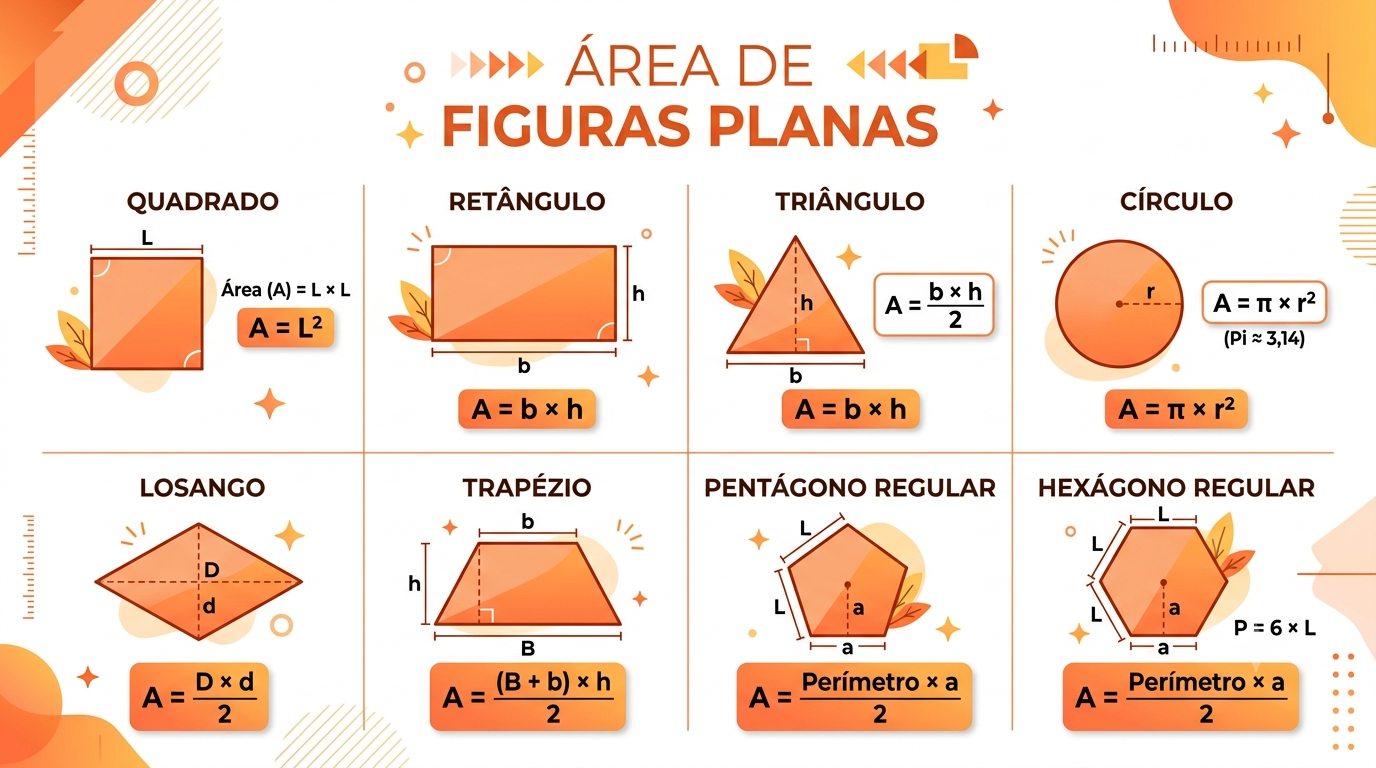
\includegraphics[width=\paperwidth]{slide_02_contracapa.png}}
            \begin{frame}[plain]                
            \end{frame}
        }

    \begin{frame}{O que é Área? O que é Perímetro?} %frame01
        \begin{columns}[T]
            \begin{column}{0.3\textwidth}
                \centering
                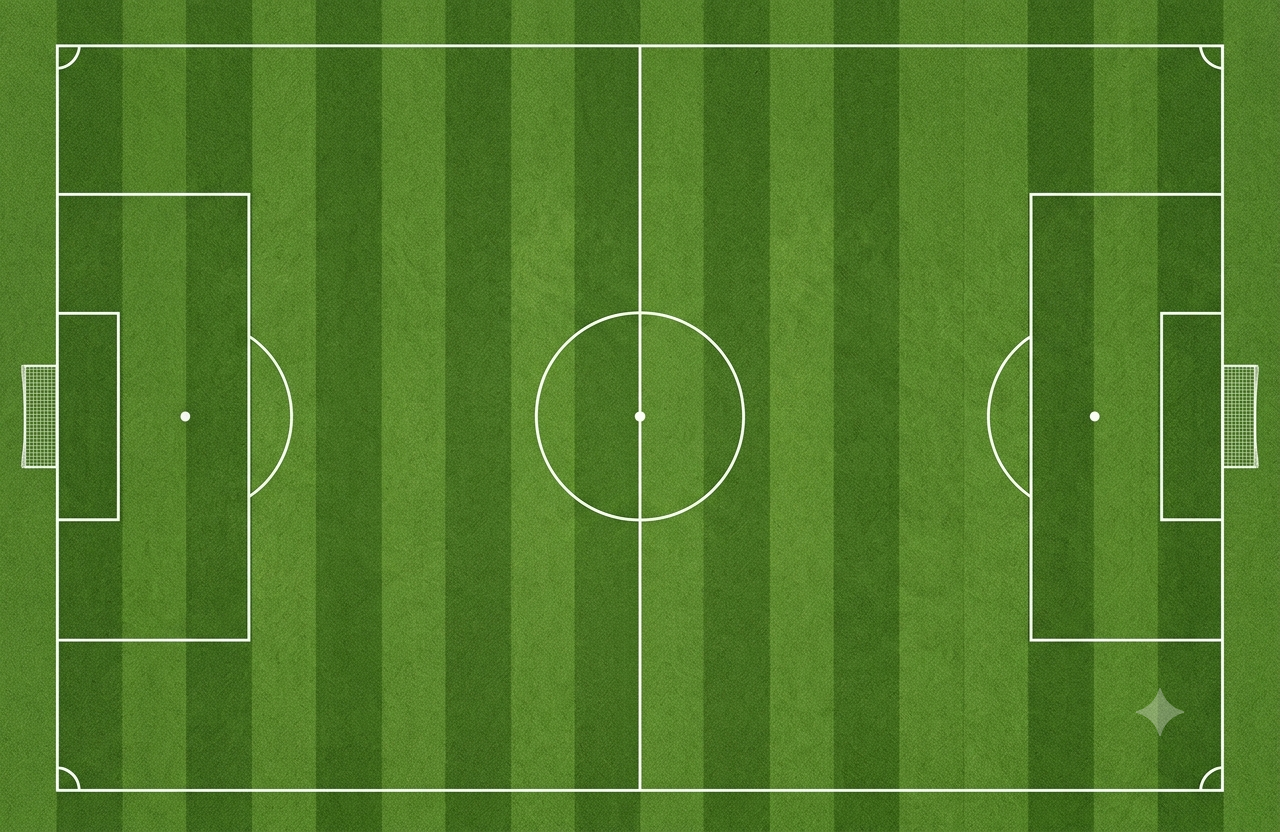
\includegraphics[angle=90, width=.7\textwidth]{slide_campo_futebol.png}

                \begin{cardPrincipal}[title=Unidades de Medida, width=\textwidth]
                    \textbf{Perímetro: } m, km, cm, dm, etc;
                    
                    \textbf{Área: } m², km², cm², dm², etc.
                \end{cardPrincipal}
            \end{column}
            \begin{column}{.65\textwidth}
                \begin{column}{.4\textwidth}
                    \centering
                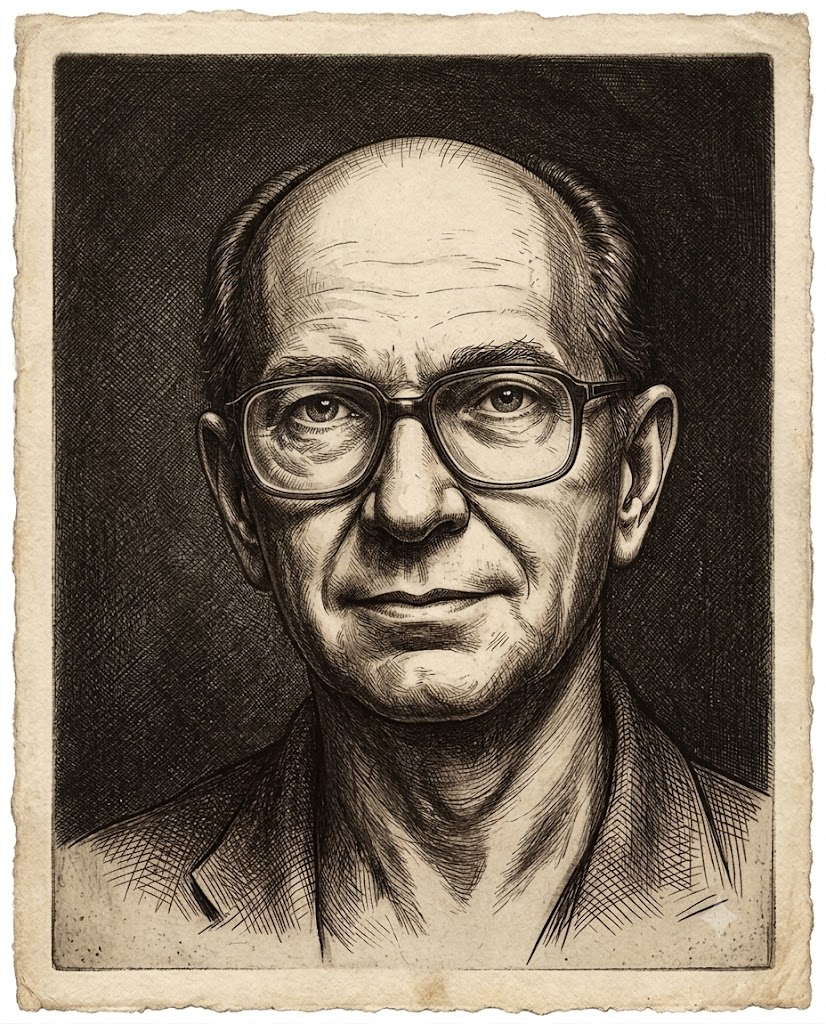
\includegraphics[width=\textwidth]{elon_lages_lima.png}
                \end{column}
                \begin{column}{.55\textwidth}
                    \vspace{1em}
                    O matemático alagoano \textbf{Elon Lages} Lima define muito bem os conceitos de Perímetro e Área.

                    Em linhas gerais, ele relaciona \textbf{Perímetro} ao comprimento, a uma linha. No caso de \textit{polígonos} é a linha do contorno.

                    A \textbf{Área}, por outro lado, é determinada por um número real \textit{não-negativo}, associado à superfície de uma figura. 
                \end{column}
                \vspace{1em}

                Podemos considerar, então, que por merdir superfícies, a área opera com duas dimensões (comprimento e largura, largura e altura, etc).

                Assim sendo, pense que a unidade da área pode ser considerada como um quadrado de lado 1.
            \end{column}
        \end{columns}    
    \end{frame}

    \begin{frame}{Propriedades Gerais da Área}
        \vspace{1.2em}
            \begin{columns}[T]
                \begin{column}{.4\textwidth}
                    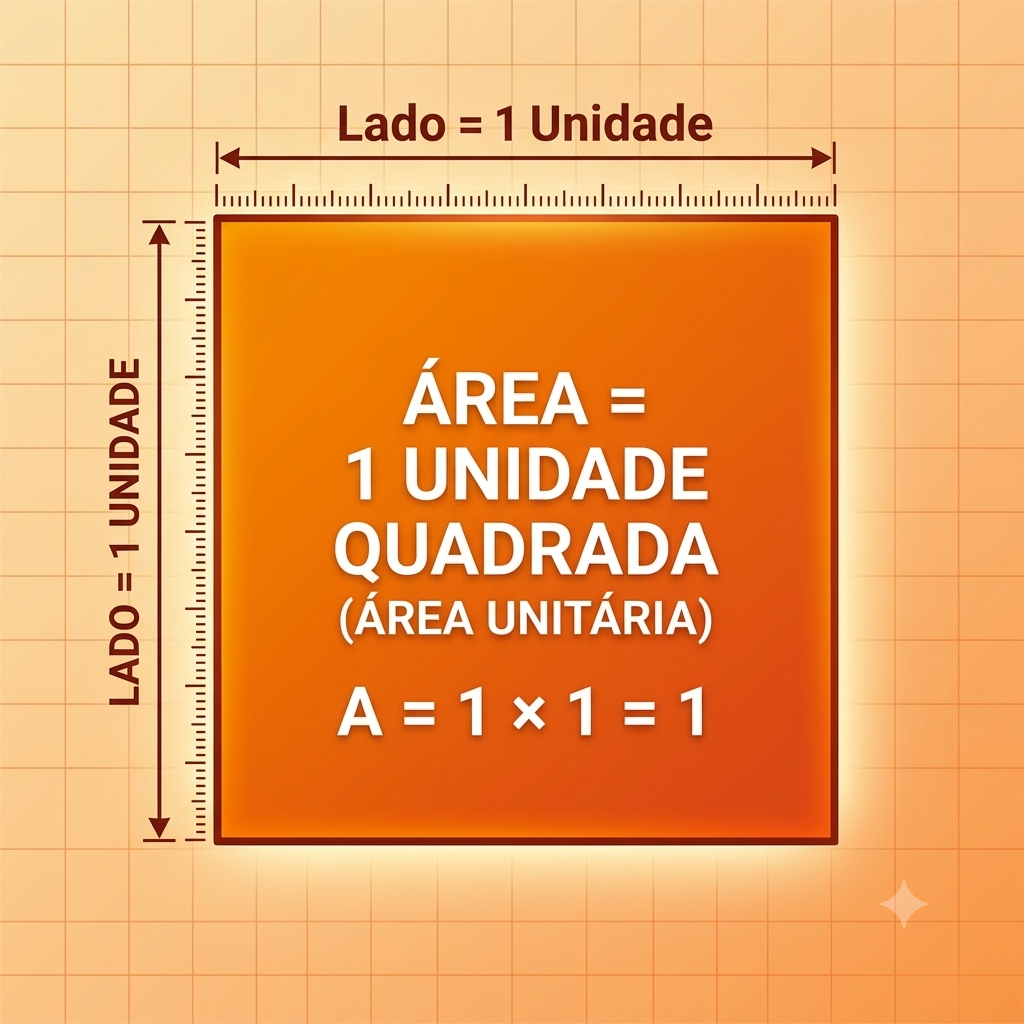
\includegraphics[width=\textwidth]{slide_area_fundamental.png}
                \end{column}
                \begin{column}{0.6\textwidth}
                    \begin{center}
                        \begin{itemize}
                            \item \textbf{Unidade de área:} Se $P$ é um quadrado de lado unitário, então $\text{área de }P = 1$;
                            \item Polígonos \textbf{congruentes} possuem áreas iguais;
                            \item Se um polígono $P$ pode ser dividido em duas ou mais regiões, a área de $P$ é a \textbf{soma das áreas} das regiões.
                        \end{itemize}

                        \vspace{1em}
                        \large{\textbf{Área do Retângulo}}
                        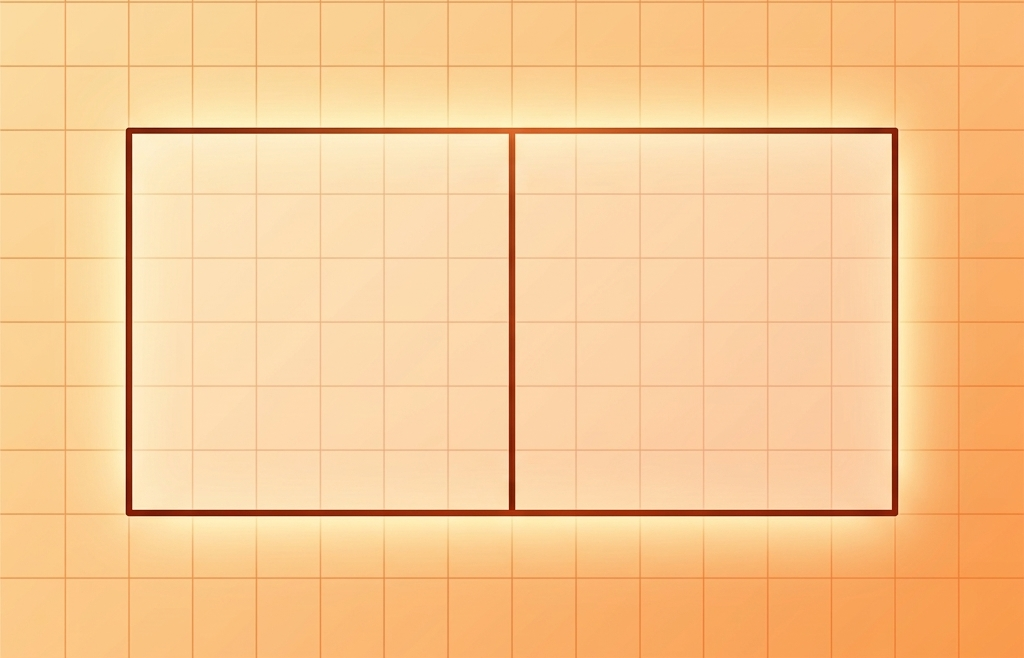
\includegraphics[width=.7\textwidth]{slide_retangulo_doisquadrados.png}
                    \end{center}
                \end{column}
            \end{columns}
    \end{frame}    

    \begin{frame}%Área do Triângulo
        \frametitle{Áreas de Figuras Mais Comuns --- Triângulo}
        Podemos não apenas usar a soma de áreas, para encontrarmos a área de outras figuras, como também podemos \textbf{decompor} um área em figuras menores. Como no caso da área do triângulo.
        \vspace{1em}
        \begin{columns}[T]
            \begin{column}{0.6\textwidth}
                \centering
                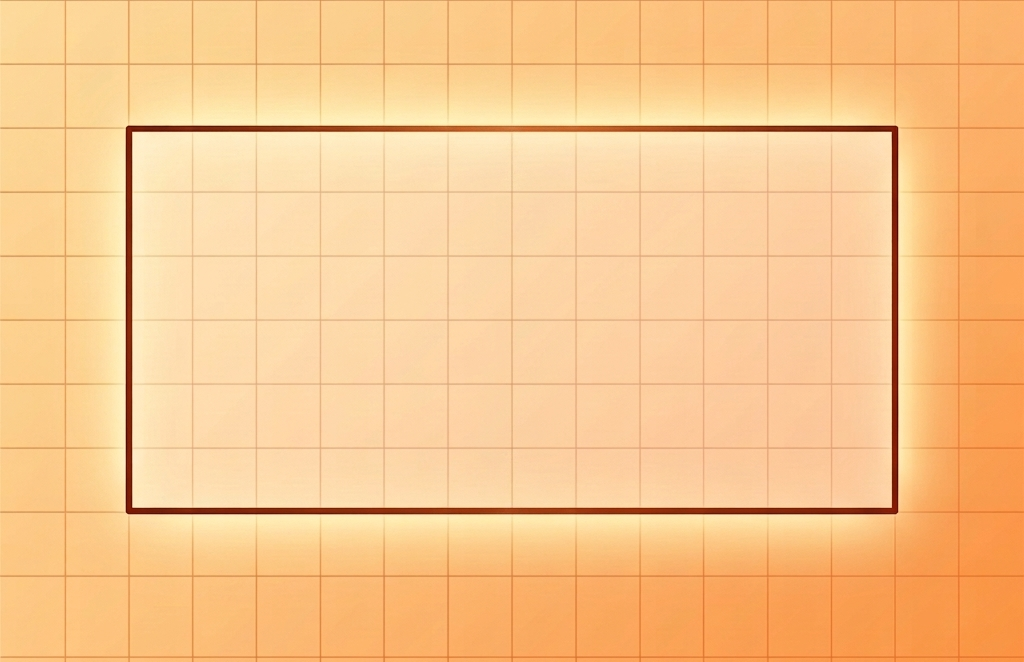
\includegraphics[width=.62\textwidth]{slide_area_retangulo.png}
            \end{column}

            \begin{column}{0.4\textwidth}
                Já definimos a área de um retângulo como o produto de sua \textit{base} por sua \textit{altura}.
                
                Podemos decompor um retângulo em duas regiões triangulares, para definirmos \textbf{a área de um triângulo}.
            \end{column}
        \end{columns}
        \vspace{1em}

        \begin{cardPrincipal}[title=Altura do triângulo]
                A altura de um triângulo é o segmento de reta perpendicular à reta suporte de sua base, traçado a partir de seu vértice oposto. Não necessariamente será um segmento interno ao triângulo.
        \end{cardPrincipal}
    \end{frame}

    \begin{frame}%Área de Paralelogramos
        \frametitle{Áreas de Figuras Mais Comuns --- Paralelogramos \& Trapézios}
        Prosseguindo com a estratégia de \textbf{decompor} figuras para deduzirmos suas áreas, ganhamos agora um grande aliado: calcular a área de polígonos convexos é \textit{dividí-los} em triângulos.

        Vejamos a estratégia aplicada às áreas do paralelogramo e do trapézio:

        \vspace{1em}
        \begin{columns}[T]
            \begin{column}{.5\textwidth}
                \centering
                \large \textbf{Área do Paralelogramo}
                \begin{figure}
                    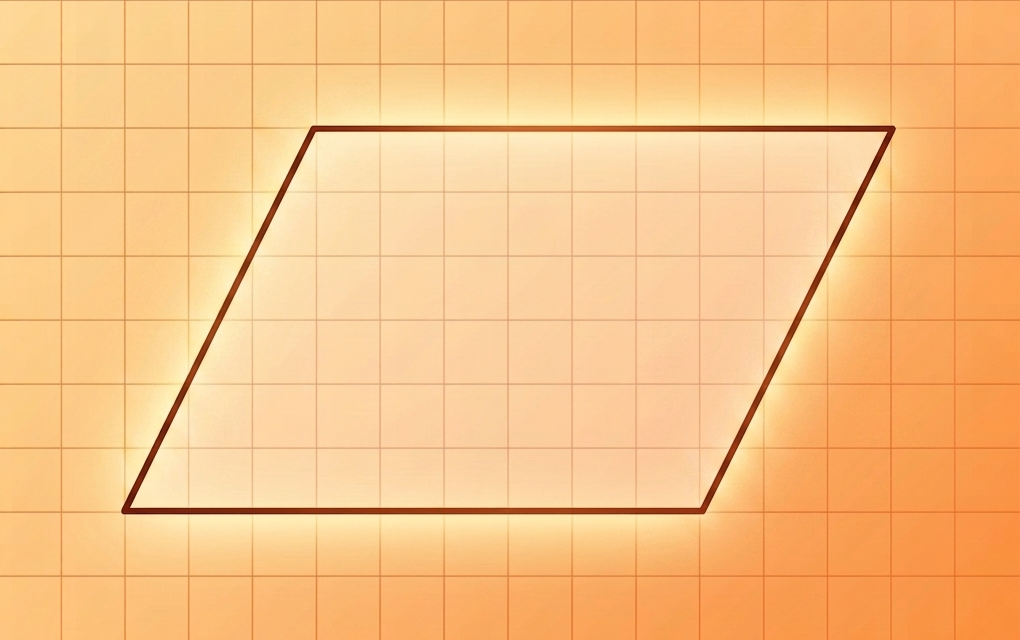
\includegraphics[width=.8\textwidth]{slide_area_paralelogramo.png}
                \end{figure}
                \begin{cardPrincipal}[width=.8\textwidth]
                    \[
                    A = B \cdot h
                    \]
                \end{cardPrincipal}
            \end{column}
            \begin{column}{.5\textwidth}
                \centering
                \large \textbf{Área do Trapézio}
                \begin{figure}
                    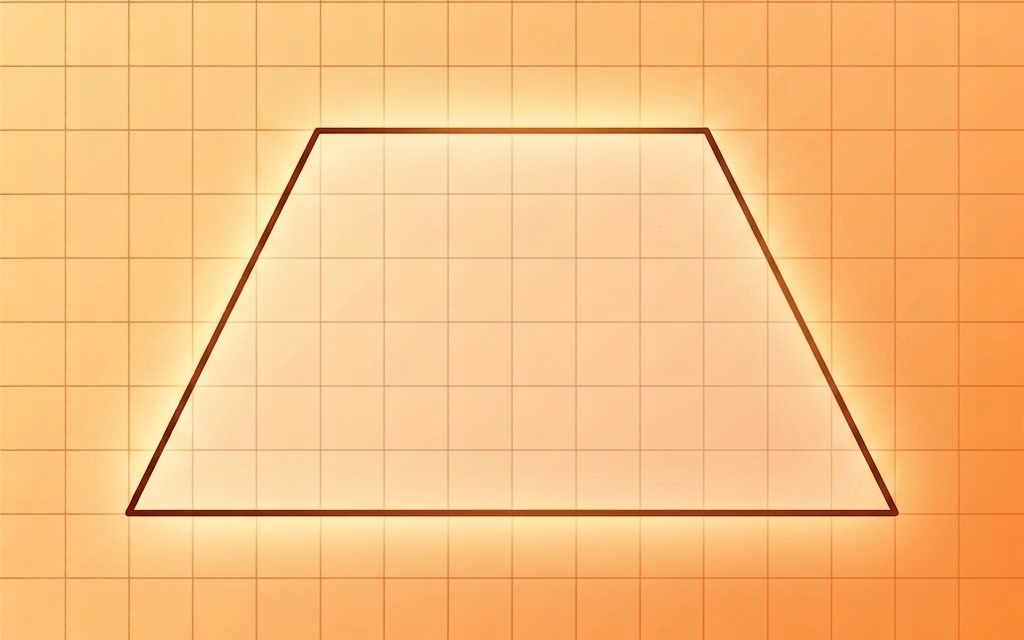
\includegraphics[width=.8\textwidth]{slide_area_trapezio.png}
                \end{figure}
                \begin{cardPrincipal}[width=.8\textwidth]
                    \centering
                    $A = \frac{(B+b)\cdot h}{2}$
                \end{cardPrincipal}
            \end{column}
        \end{columns}
    \end{frame}

    \begin{frame}%Área de Polígonos Regulares
        \frametitle{Área de Polígonos Regulares}
        \vspace{1.2em}
        \begin{columns}[T]
            \begin{column}{.5\textwidth}
                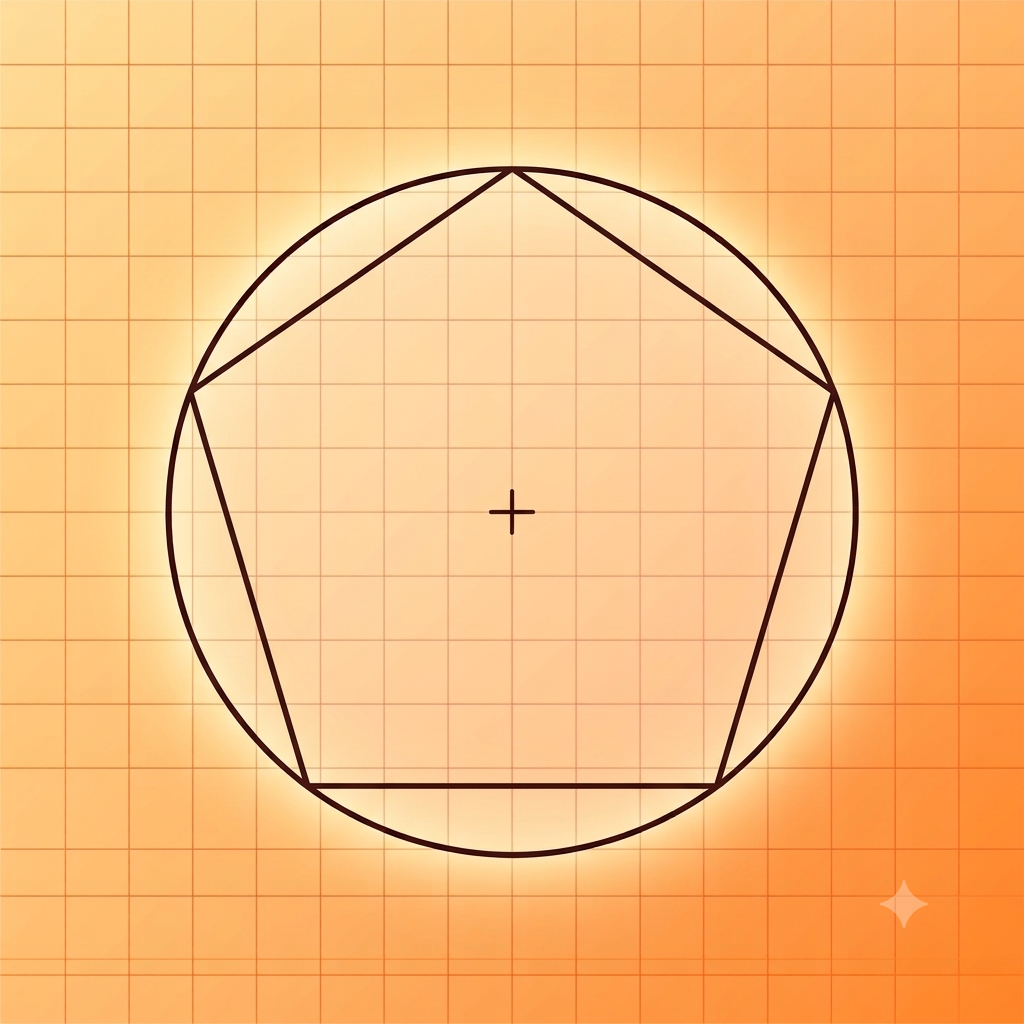
\includegraphics[width=.9\textwidth]{slide_pentagono.png}
            \end{column}
            \begin{column}{.5\textwidth}
                A mesma estratégia de decomposição de áreas pode ser aplicada a qualquer \textbf{polígono convexo}. No caso de polígonos \textbf{regulares}, 
            \end{column}
        \end{columns}
    \end{frame}

    \begin{frame} %Perímetros de Polígonos
        \frametitle{Perímetro de Polígonos}
        O cálculo do perímetro de uma figura é relativamente simples: no caso de polígonos, basta somar os valores dos lados da figura.
        Esse vamos representa o comprimento dos lados da figura, caso fossem colocados em linha, um após o outro, formando um segmento de reta.
        \vspace{.3em}
        \begin{columns}[T]
            \begin{column}{.35\textwidth}
                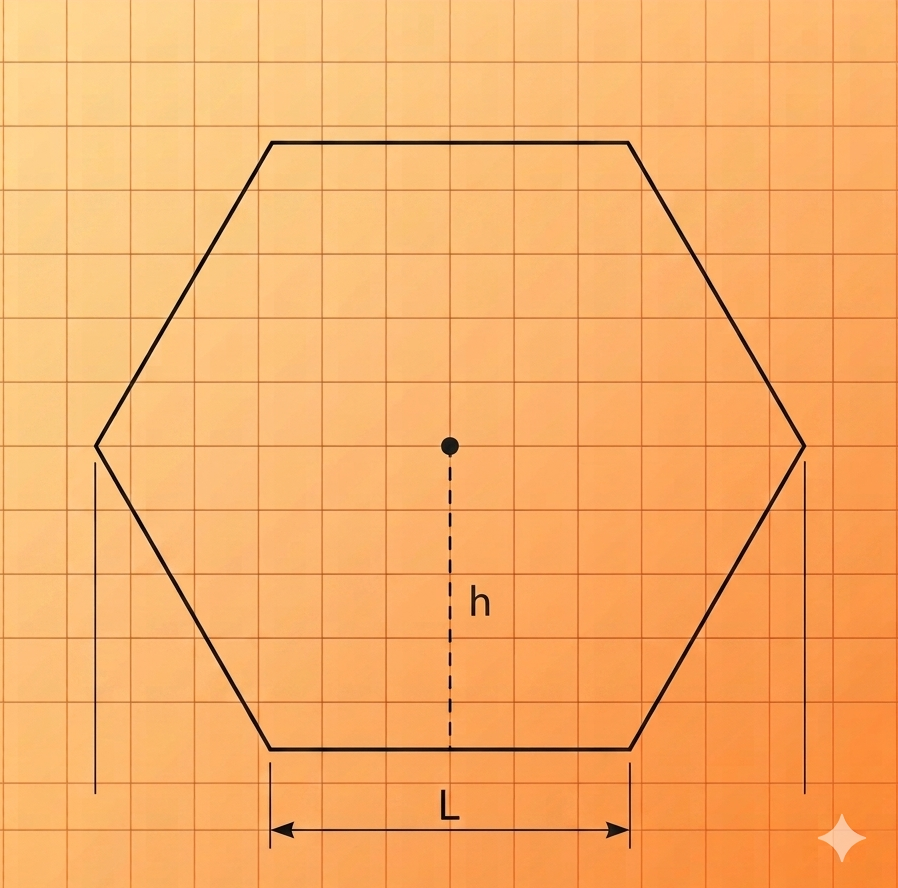
\includegraphics[width=\textwidth]{slide_permitroxarea.png}
            \end{column}
            \begin{column}{.6\textwidth}
                Podemos estabelecer uma \textbf{relação entre o perímetro de polígonos regulares e sua área}. No exemplo ao lado, temos um hexágono com lado de medida \textbf{L}. Seu perímetro é \textbf{6L}. Se dividirmos em seis triângulos tomando \textbf{L} como base, a altura de cada um será o segmento \textbf{h}. E a área da figura será:

                $$
                    \text{Área}_{\text{hexágono}} = \frac{6L \cdot h}{2}
                $$

                \begin{cardPrincipal}[width=\textwidth]
                \begin{columns}[c]
                    \begin{column}{.5\textwidth}
                            \[
                            \text{Área} = \frac{p}{2} \cdot h
                            \]
                    \end{column}
                    \begin{column}{.5\textwidth}
                        \textbf{metade do perímetro }$\left( \frac{p}{2} \right)$ \textbf{vezes a o segmento que vai do centro da figura ao ponto médio de um de seus lados}$\left( h \right)$.
                    \end{column}
                \end{columns}
            \end{cardPrincipal}
            \end{column}
        \end{columns}
    \end{frame}

    \begin{frame} % Perímetro de Círculos
        \frametitle{Perímetro de Círculos}
        A idéia do perímetro de um círculo é a seguinte: imagine um círculo formado por um fio. Imagine que posamos cortar esse fio e esticá-lo em linha reta, sem que ele se deforme, para medirmos o comprimento da circunferência.
        Esse comprimento sempre será \textbf{o produto do diâmetro por um valor constante chamado pi}.
        \vspace{1em}
        \begin{columns}[T]
            \begin{column}{.4\textwidth}
                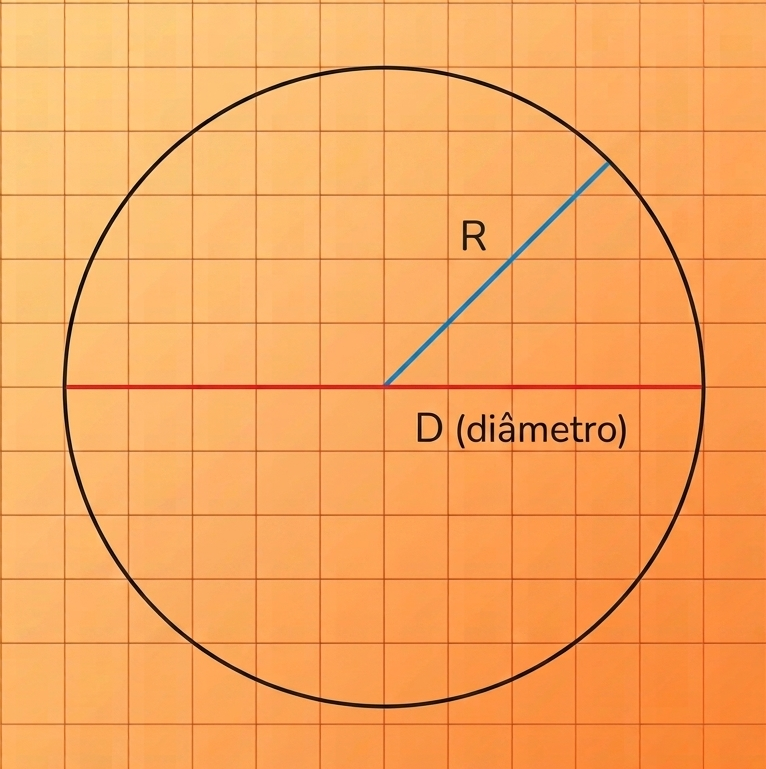
\includegraphics[width=\textwidth]{slide_circulo_raio_diametro.png}
            \end{column}
            \begin{column}{.5\textwidth}
 
                \begin{cardPrincipal}[title=Relação Raio x Diâmetro]
                    O \textbf{raio$(r)$} é a medida que vai do centro a um ponto da circunferência. O \textbf{diâmetro$(d)$} corresponde a \textbf{duas vezes o raio}. $d = 2 \cdot r$
                \end{cardPrincipal}
                \vspace{0.6em}
                \begin{cardPrincipal}[title=Comprimento(C) da Circunferência]
                    \[
                        C = 2 \cdot \pi r
                    \]
                \end{cardPrincipal}
            \end{column}
        \end{columns}
    \end{frame}

    \begin{frame} % Área de Círculos
        \frametitle{Área de Círculos}
        Embora não possamos dividir a área do círculo em triângulos perfeitos, podemos utilizar essa ideia em combinação com a idéia da área relacionada à metade do perímetro.
        \vspace{.6em}
        \begin{columns}[T]
            \begin{column}{.35\textwidth}
                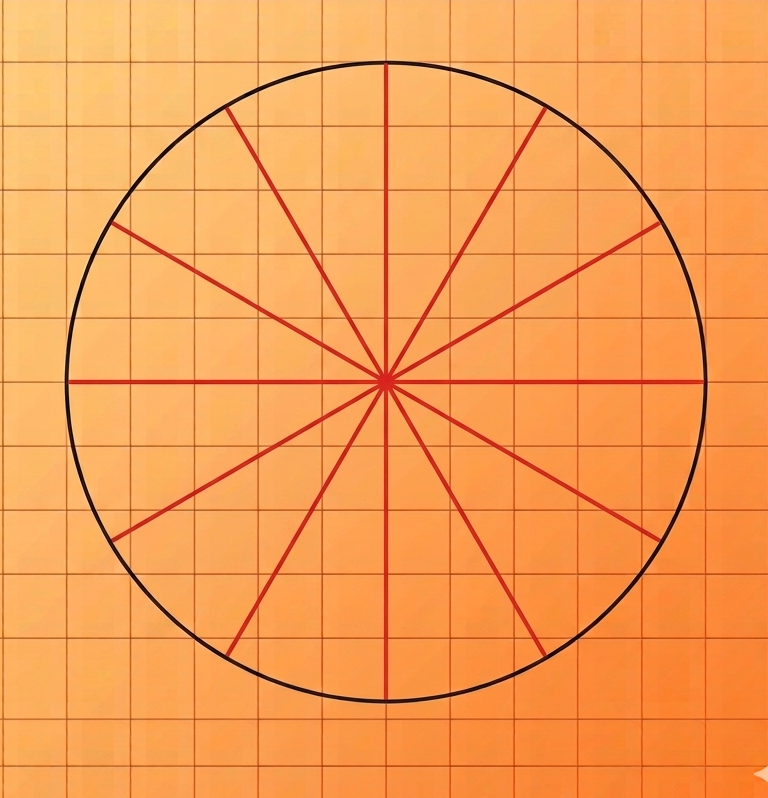
\includegraphics[width=\textwidth]{slide_area_circulo.png}
            \end{column}
            \begin{column}{.65\textwidth}
                Perceba na imagem ao lado que podemos dividir um círculo em fatias. Cada uma delas se aproxima de um triângulo, com a altura definida por um raio.

                A cada vez que aumentamos o número de fatias, elas se aproximarão de triâgulos tendo o raio como altura.

                Então, se pudéssemos dividir em infinitos triângulos: a altura seria igual ao raio do círculo.

                Por outro lado, o semiperímetro do círculo é:
                
                    \[
                        \frac{p}{2} = \frac{2\cdot \pi \cdot r}{2} = \pi\cdot r
                    \]
                
                Fazendo o produto do semiperímetro do círculo pelo raio:

                \centering
                \begin{cardPrincipal}[title=Área do Círculo, width=.8\textwidth]
                    \[
                        \text{Área}_\text{círculo} = \pi \cdot r \cdot r = \pi \cdot r^{2}
                    \]
                \end{cardPrincipal}
            \end{column}
        \end{columns}
    \end{frame}
    

%----------------------------------------------
%              EXERCICIOS
%----------------------------------------------

    \begin{frame} %Exercício01
        \frametitle{Exercícios}
        \begin{columns}
            \begin{column}{.9\textwidth}
                1.~\textbf{(ENEM-2018): }Um brinquedo chamado pula-pula, quando visto de cima, consiste de uma cama elástica com contorno em formato de um hexágono regular.
                \begin{columns}
                    \begin{column}{0.4\textwidth}
                        \begin{figure}
                            \centering
                            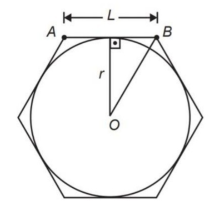
\includegraphics[width=1\textwidth]{figura_exe01.png}
                        \end{figure}
                    \end{column}

                    \begin{column}{0.7\textwidth}
                        
                        Se a área do círculo inscrito no hexágono é $3\pi$ metros quadrados, então a área do hexágono, em metro quadrado, é
                        \vspace{0.2cm}
                        \begin{enumerate}[a.]
                            \item $9$
                            \item $6\sqrt{3}$
                            \item $9\sqrt{2}$
                            \item $12$
                            \item $12\sqrt{3}$
                            % letra B
                        \end{enumerate}

                    \end{column}
                \end{columns}
            \end{column}
        \end{columns}
    \end{frame}

    \begin{frame} %Exercício 02
        \frametitle{Exercícios}
        \begin{columns}
            \begin{column}{.9\textwidth}
                2.~\textbf{(ENEM-2017): }A figura traz o esboço da planta baixa de uma residência. Algumas medidas internas dos cômodos estão indicadas. A espessura de cada parede externa da casa é 0,20 m e das paredes internas, 0,10 m.

                \begin{columns}
                    \begin{column}{0.4\textwidth}
                        \begin{figure}
                            \centering
                            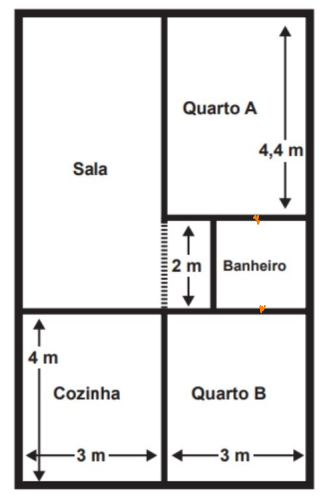
\includegraphics[width=0.8\textwidth]{figura_plantabaixa.png}
                        \end{figure}
                    \end{column}
                    \begin{column}{0.5\textwidth}
                        \vspace{0.2cm}

                        Sabe-se que, na localidade onde se encontra esse imóvel, o Imposto Predial Territorial Urbano (IPTU) é calculado conforme a área construída da residência. Nesse cálculo, são cobrados R\$ 4,00 por cada metro quadrado de área construída.

                        O valor do IPTU desse imóvel, em real, é
                        \begin{enumerate}[a.]
                            \item 250,00
                            \item 250,80
                            \item 258,64
                            \item 276,48
                            \item 286,00
                            % letra e
                        \end{enumerate}

                    \end{column}
                \end{columns}
            \end{column}
        \end{columns}
    \end{frame}

    \begin{frame} %Exercício 03
        \frametitle{Exercícios}
        \begin{columns}
            \begin{column}{.9\textwidth}
                3.~\textbf{(ENEM-2024): }Um sistema de polias circulares e correias é um dos mecanismos responsáveis pela transmissão de movimento em máquinas rotativas. O manual de um motor traz uma figura representando um sistema composto por duas polias e uma correia de transmissão, tensionada e perfeitamente ajustada sobre as polias, de modo a não apresentar folgas nos contatos com as polias. Considere que as partes dessa correia que não ficam em contato com as polias são representadas por segmentos de reta tangentes às polias.

                Para substituição dessa correia, é necessária a especificação de seu comprimento.

                Considere 3 como valor aproximado para $\pi$.

                A medida do comprimento dessa correia, em centímetro, é
              
                \begin{columns}
                    \begin{column}{0.6\textwidth}
                        \begin{table}
                            \begin{figure}
                                \centering
                                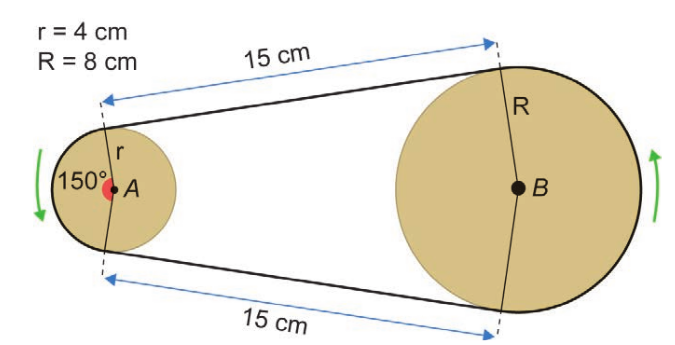
\includegraphics[width=.75\textwidth]{figura_polia.png}
                            \end{figure}
                        \end{table}
                    \end{column}
                    \begin{column}{0.35\textwidth}
                        \begin{enumerate}[a.]
                            \item 50
                            \item 60
                            \item 66
                            \item 68
                            \item 72
                            % letra D
                        \end{enumerate}

                    \end{column}
                \end{columns}
            \end{column}
        \end{columns}
    \end{frame}

    \begin{frame} %Exercicio 04
        \frametitle{Exercícios}
        \begin{columns}
            \begin{column}{.9\textwidth}
                4.~\textbf{(ENEM-2024): }Uma microempresa pretende fabricar pipas para vender no próximo verão. Um modelo de pipa está representado pelo quadrilátero ABCD.
                
                Nessa representação, os segmentos AB, BC e CE medem, respectivamente, 20 cm, 34 cm e 30 cm. Além disso, E pertence ao segmento AC e é ponto médio do segmento BD.

                A medida da área, em centímetro quadrado, desse modelo de pipa é 
                \vspace{1em}
                
                \begin{columns}[T]
                    \centering
                    \begin{column}{0.55\textwidth}
                        \centering
                        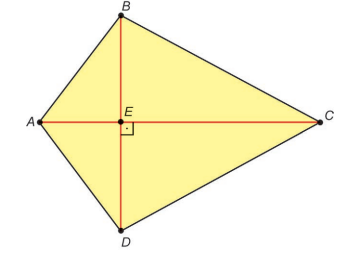
\includegraphics[width=.8\textwidth]{figura_pipa.png}
                    \end{column}
                    \begin{column}{0.3\textwidth}
                        \begin{enumerate}[a.]
                            \item 58
                            \item 96
                            \item 108
                            \item 184
                            \item 672
                            % letra E
                        \end{enumerate}
                    \end{column}
                    \begin{column}{0.5\textwidth}
                        
                    \end{column}
                \end{columns}
            \end{column}
        \end{columns}
    \end{frame}

    \begin{frame} %Exercicio 05
        \frametitle{Exercícios}
        \begin{columns}
            \begin{column}{.9\textwidth}
                5.~\textbf{(ENEM-2024): }Um jardineiro dispõe de k metros lineares de cerca baixa para fazer um jardim ornamental. O jardim, delimitado por essa cerca, deve ter a forma de um triângulo equilátero, um quadrado ou um hexágono regular.
                
                A escolha será pela forma que resulte na maior área. O jardineiro escolherá a forma de um 

                \begin{columns}
                    \begin{column}{.1\textwidth}
                        
                    \end{column}
                    \begin{column}{.9\textwidth}
                         
                        \begin{enumerate}[a.]
                            \item hexágono regular, pois a área do jardim, em metro quadrado, será $\displaystyle \frac{k^2 \sqrt{3}}{24} $
                            \item hexágono regular, pois a área do jardim, em metro quadrado, será $\displaystyle \frac{3k^2\sqrt{3}}{2}$
                            \item quadrado, pois a área do jardim, em metro quadrado, será $\displaystyle \frac{k^2}{16}$
                            \item triângulo equilátero, pois a área do jardim, em metro quadrado, será $\displaystyle \frac{k^2 \sqrt{3}}{36}$
                            \item triângulo equilátero, pois a área do jardim, em metro quadrado, será $\displaystyle \frac{k^2 \sqrt{3}}{4}$
                            % letra A
                        \end{enumerate}
                    \end{column}
                    \begin{column}{0.5\textwidth}
                        
                    \end{column}
                \end{columns}
            \end{column}
        \end{columns}
    \end{frame}
    
    \begin{frame} %Exercicio 06
        \frametitle{Exercícios}
        \begin{columns}
            \begin{column}{.9\textwidth}
                6.~\textbf{(ENEM-2023): }Uma empresa de publicidade está criando um logotipo que tem o formato indicado na figura. O círculo menor está inscrito no quadrado ABCD, e o círculo maior circunscreve o mesmo quadrado. Considere S1 a área do círculo menor e S2 a área do círculo maior. 
                \vspace{1.2em}
                \begin{columns}[T]
                    \begin{column}{0.4\textwidth}
                        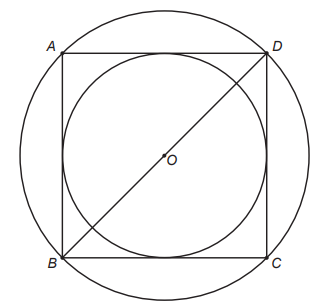
\includegraphics[width=\textwidth]{figura_questao6.png}
                    \end{column}
                    \begin{column}{0.5\textwidth}
                        A razão da área do círculo maior para o círculo menor é igual a 
                        \begin{enumerate}[a.]
                            \item $\sqrt{2}$
                            \item $\frac{1}{2}$
                            \item 2
                            \item 8
                            \item 16
                            % letra E
                        \end{enumerate}
                    \end{column}
                \end{columns}
            \end{column}
        \end{columns}
    \end{frame}
\end{document}